\documentclass{standalone}
\usepackage{tikz}
\usepackage{amsmath}
\usetikzlibrary{matrix,chains,positioning,decorations.pathreplacing,arrows}
\usetikzlibrary{positioning, calc, chains}
\begin{document}


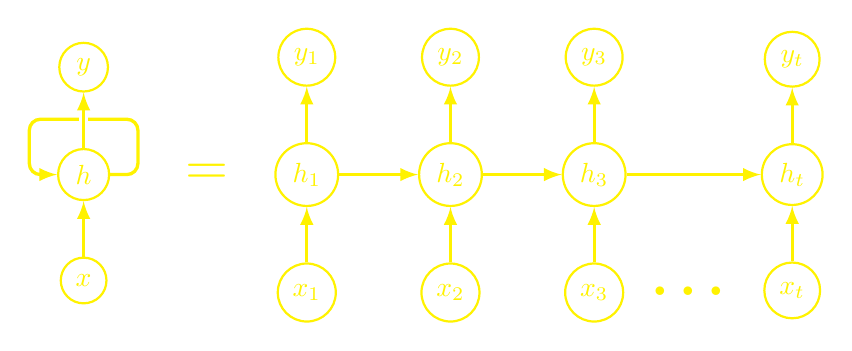
\begin{tikzpicture}[draw=yellow, item/.style={circle,draw,thick,align=center},
itemc/.style={item,on chain,join}]
\begin{scope}[start chain=going right,nodes=itemc,every
join/.style={-latex,very thick},local bounding box=chain]
\path node[color=yellow] (h1) {$h_1$} node[color=yellow]  (h2) {$h_2$} node[color=yellow]  (h3) {$h_3$} node[xshift=2em, color=yellow] (ht)
{$h_t$};
\end{scope}
\node[left=1em of chain,scale=2, color=yellow] (eq) {$=$};
\node[left=2em of eq,item, color=yellow] (AL) {$h$};
\path (AL.west) ++ (-1em,2em) coordinate (aux);
\draw[very thick,-latex,rounded corners, color=yellow] (AL.east) -| ++ (1em,2em) -- (aux) 
|- (AL.west);
\foreach \T in {1,2,3,t} 
{\draw[very thick,-latex] (h\T.north) -- ++ (0,2em)
	node[above,item, color=yellow] (y\T) {$y_\T$};
	\draw[very thick,latex-] (h\T.south) -- ++ (0,-2em)
	node[below,item, color=yellow] (x\T) {$x_\T$};}
\draw[white,line width=0.8ex] (AL.north) -- ++ (0,1.9em);
\draw[very thick,-latex] (AL.north) -- ++ (0,2em)
node[above,item, color=yellow] {$y$};
\draw[very thick,latex-] (AL.south) -- ++ (0,-2em)
node[below,item, color=yellow] {$x$};
\path (x3) -- (xt) node[color=yellow, midway,scale=2,font=\bfseries] {\dots};



\end{tikzpicture}



\end{document}